\documentclass[runningheads]{llncs}

\usepackage[T1]{fontenc}
\usepackage[utf8]{inputenc}
\usepackage{amssymb,amsfonts}
\vbadness=10000
\usepackage{graphicx}
\usepackage{booktabs}
\usepackage{tabularx}
\usepackage{array}
\usepackage{makecell}
\usepackage{multirow}
\usepackage{xcolor}
\usepackage{bm}
\usepackage{url}
\usepackage[hidelinks]{hyperref}
\usepackage{microtype}
\newcommand{\operatorname}[1]{\mathop{\mathrm{#1}}}

\newcolumntype{Y}{>{\raggedright\arraybackslash}X}
\newcolumntype{C}{>{\centering\arraybackslash}X}
\newcommand{\aes}{AES-RARR}
\newcommand{\vsr}{\mathrm{VSR}}
\newcommand{\ttr}{\mathrm{TTR}}
\newcommand{\rap}{\mathrm{RAP}}

\title{Active Evidential Sensing for Occlusion-Robust Maritime Search and Rescue}
\titlerunning{Active Evidential Sensing for Maritime SAR}

\author{Nguyen Trinh Quy\inst{1} \and Thu Le\inst{1} \and Tran Thanh Vu\inst{1} \and Pham Nguyen Khanh Nguyen\inst{1}}
\authorrunning{N. T. Quy et al.}
\institute{FPT University HCM, Ho Chi Minh City, Vietnam}

\begin{document}
\maketitle

\begin{abstract}
Unmanned aerial vehicles are increasingly used in maritime search and rescue because they can cover large sea areas without placing flight crews at risk. Current vision-based systems, however, often treat detections and class probabilities as deterministic observations. This assumption is fragile when waves, spray, glare, and altitude changes obscure a victim. A drowning victim can therefore be assigned a low or ambiguous posture score while the rescue scheduler moves to easier targets. This paper studies that failure case through \aes, an active sensing and rescue-routing framework for UAV-assisted maritime SAR. The framework represents posture uncertainty with evidential deep learning, propagates spatial and epistemic uncertainty into a drift-aware Kalman tracker, and triggers a lower-altitude verification pass when an observation is both risky and uncertain. Confirmed tracks are then ranked by a risk-averse priority score that combines posture risk, uncertainty, estimated travel time, and survival decay. Since public maritime UAV datasets do not provide frame-level distress labels, the present study evaluates the closed loop in simulation using a distance- and occlusion-dependent evidential proxy. Across 100 Monte Carlo trials with three-victim scenarios and 30\% initial occlusion, \aes improves worst-case victim survival rate from $0.30 \pm 0.11$ for a deterministic expected-risk baseline to $0.52 \pm 0.08$, while reducing catastrophic failure rate from 52\% to 6\%. The results support uncertainty-triggered verification as a practical mechanism for reducing delayed rescue decisions under wave occlusion, while also identifying the data requirements needed for deployment with a trained visual model.
\keywords{Maritime search and rescue \and UAV \and evidential deep learning \and active sensing \and uncertainty-aware tracking \and rescue routing}
\end{abstract}

\section{Introduction}

Maritime search and rescue (mSAR) is a time-constrained decision problem. Survival after immersion depends on cold shock, swim failure, cold incapacitation, hypothermia, sea state, clothing, flotation support, and the time needed for rescue assets to reach the casualty \cite{golden2002,tipton2011,bierens2016,iamsar2019}. UAVs provide useful sensing capacity in this setting because they can rapidly inspect broad search regions using electro-optical and thermal cameras, and they can transmit visual evidence to rescue coordinators without exposing crews to unnecessary risk \cite{queralta2020,messmer2024holistic}.

Recent datasets and UAV vision systems have improved detection and tracking of people, swimmers, boats, and other objects in maritime imagery \cite{varga2022seadronessee,ngo2026drowning}. These systems are useful for locating targets, but the routing decision after detection remains difficult. A rescue asset must decide which victim to verify first and which victim to rescue first. A nearest-first policy can be unsafe when the closest person is stable and a farther person is drowning. A deterministic expected-risk policy can also be unsafe when the most urgent victim is partly occluded by waves and receives an uncertain or misleading posture estimate.

The problem is not only classification error. It is the absence of a decision mechanism that treats uncertainty as a reason to gather more evidence. Standard Softmax networks are known to be poorly calibrated in many settings \cite{guo2017calibration}. In maritime imagery, the same target can look different across altitude, viewpoint, wave phase, reflection, and partial submersion. Predictive uncertainty should therefore be separated into aleatoric uncertainty, which reflects observation noise, and epistemic uncertainty, which reflects lack of reliable evidence or model knowledge \cite{kendall2017uncertainties}. If the rescue scheduler ignores this distinction, an occluded drowning victim may be postponed precisely because the system is unsure. We refer to this as the silent drowning failure mode.

This paper presents \aes, an active evidential sensing and risk-averse rescue-routing framework. The framework combines four components. First, a multimodal detector is designed to output bounding boxes, spatial uncertainty, and evidential posture parameters rather than only point estimates. Second, detections are projected to the sea surface and tracked with a Kalman filter whose measurement covariance increases when spatial or epistemic uncertainty is high. Third, uncertain high-risk observations trigger an active sensing branch in which the UAV descends from search altitude to verification altitude. Fourth, confirmed tracks are ranked by a risk-averse priority score that accounts for posture risk, uncertainty, survival decay, and travel distance.

The present work is a simulation study. This qualification is important because widely used public maritime UAV datasets do not contain the four distress-state labels required to train a real posture model. SeaDronesSee, for example, provides categories such as person, swimmer, life jacket, boat, and buoy, but not frame-level labels such as drowning, floating, swimming, or PFD floater \cite{varga2022seadronessee}. For this reason, the experiments use an evidential proxy oracle whose output becomes uncertain under occlusion and more class-specific at close range. The objective is not to claim deployment readiness, but to evaluate whether the closed-loop decision rule is useful once such uncertainty estimates are available.

The contribution of this paper is threefold. It formalizes a wave-occlusion failure case in UAV-assisted mSAR where deterministic rescue routing can postpone high-risk victims. It proposes a closed-loop active sensing mechanism that uses evidential uncertainty to decide when the UAV should gather more information. It evaluates the resulting rescue decisions in Monte Carlo simulation against deterministic, no-branch, static-tracking, and distance-based baselines, reporting both mean performance and worst-case survival outcomes.

\section{Related Work}

\subsection{UAV-Based Maritime Search and Rescue}

Early operational SAR planning relied on search theory, probability of containment, probability of detection, and drift models to allocate effort over uncertain regions \cite{koopman1980search,stone2016optimal,breivik2008sar}. These models remain central in maritime operations, but they were developed mainly for search-area planning rather than onboard visual decision making. UAVs add high-resolution visual observations, but they also introduce perception failures that depend on altitude, camera angle, target size, wave state, and communication bandwidth.

SeaDronesSee provided an important benchmark for UAV-based maritime visual perception \cite{varga2022seadronessee}. It made large-scale aerial imagery available for detection and tracking research, but its annotations do not directly encode victim urgency. AutoSOS studied multi-UAV support for maritime SAR with lightweight AI and edge processing \cite{queralta2020}. Messmer and colleagues considered holistic UAV-assisted mSAR and bandwidth-aware region prioritisation \cite{messmer2024holistic}. These works motivate integrated perception and planning, but they do not provide a closed-loop mechanism in which epistemic uncertainty changes the sensing trajectory.

Recent work by Ngo et al. studied UAV-based visual detection and tracking of drowning victims with RGB and thermal input \cite{ngo2026drowning}. That direction is close to the present problem because posture state is linked to rescue urgency. However, deterministic class probabilities remain a weak basis for safety-critical routing under occlusion. \aes therefore focuses on the missing connection between uncertainty estimation, active verification, tracking covariance, and rescue prioritisation.

\subsection{Uncertainty in Vision Models}

Bayesian deep learning distinguishes uncertainty caused by data noise from uncertainty caused by model ignorance \cite{kendall2017uncertainties}. Monte Carlo dropout approximates Bayesian inference by repeated stochastic forward passes \cite{gal2016dropout}, and deep ensembles often provide strong uncertainty estimates at the cost of multiple models \cite{lakshminarayanan2017ensembles}. Prior networks and related distributional approaches further model uncertainty by predicting distributions over class probabilities \cite{malinin2018prior}. Ovadia et al. showed that uncertainty quality can degrade under dataset shift, which is relevant to maritime imagery because occlusion, glare, and altitude changes create shifted observations \cite{ovadia2019shift}.

Evidential deep learning provides a computationally attractive alternative for edge systems because it predicts evidence parameters for a Dirichlet distribution in a single forward pass \cite{sensoy2018edl}. The total evidence controls epistemic uncertainty. When little evidence supports any class, uncertainty is high. This behavior is suitable for wave occlusion, where a target can be visible as an object but not sufficiently visible for reliable posture classification. The present study uses this formalism for decision making, while making clear that the image-based evidential detector is simulated rather than trained on a real posture dataset.

\subsection{Tracking and Active Sensing}

Kalman filtering and its multi-target extensions provide standard tools for state estimation under measurement noise \cite{kalman1960filter,barshalom2001estimation,blackman1999design}. Vision-based tracking systems such as SORT, DeepSORT, and ByteTrack demonstrate how detections can be linked over time in video \cite{bewley2016sort,wojke2017deepsort,zhang2022bytetrack}. In maritime SAR, the measurement model must also account for georeferencing error, sea-surface projection, camera altitude, and ocean-current drift.

Active sensing changes the sensor state to reduce uncertainty rather than passively accepting observations. The idea is common in robotics and planning \cite{lavalle2006planning,thrun2005probabilistic}, but it is less developed in UAV mSAR pipelines where the visual model, tracker, and rescue scheduler are often treated as separate stages. In \aes, active sensing is not a general exploration policy. It is a targeted descent action that is triggered only when the estimated uncertainty and risk suggest that a rescue decision would otherwise be unsafe.

\section{System Overview}

The closed-loop design of \aes{} is structured into two main phases: the \textit{Perception Phase} and the \textit{Decision-Making and Routing Phase} (as shown in Fig.~\ref{fig:pipeline}). The separation between these phases is defined by two levels of inputs and outputs:
\begin{itemize}
    \item \textbf{Level 1 (System-Level Inputs):} Aligned raw sensory feeds, including RGB frames $\mathbf{I}_{RGB}$ and thermal (LWIR) frames $\mathbf{I}_{Thermal}$, coupled with raw UAV telemetry $\mathbf{T}_{tel} = [\mathbf{p}_{UAV}, z_{UAV}, \boldsymbol{\theta}_{cam}]$ representing position, altitude, and camera attitude.
    \item \textbf{Level 2 (Algorithm-Level Inputs for the Decision Engine):} Features extracted by the perception module, comprising victim bounding boxes $\mathbf{b}_{i,t}$, projected geographic position estimates $\mathbf{x}_{i,t}$ with spatial covariance $\boldsymbol{\Sigma}^{geo}_{i,t}$, posture belief distributions $\mathbf{b}_{i,t,k}$, epistemic uncertainty $u_{i,t}$, expected risk $\mathbb{E}[R_i(t)]$, and logistics parameters such as distance $D_i(t)$ and estimated travel time $t_{travel,i}$.
\end{itemize}

During the \textbf{Perception Phase}, raw Level 1 inputs are processed by a fused deep network to localize bounding boxes and classify victim postures. During the \textbf{Decision-Making and Routing Phase}, the \aes{} decision engine ingests the Level 2 inputs to perform three coordinated actions:
\begin{enumerate}
    \item \textbf{Uncertainty-Aware Tracking:} Feeds projected detections and spatial/epistemic uncertainty parameters into a Kalman filter, dynamically inflating measurement noise under wave occlusion.
    \item \textbf{Active Sensing Trigger:} Evaluates expected risk and epistemic uncertainty to decide if the UAV should adjust its flight state by descending from patrol altitude ($z_{search}$) to verification altitude ($z_{verify}$).
    \item \textbf{Risk-Averse Scheduling:} Computes UCB-style priority scores to sequence the rescue path over confirmed tracks, balancing victim urgency against travel latency.
\end{enumerate}

\begin{figure}[t]
  \centering
  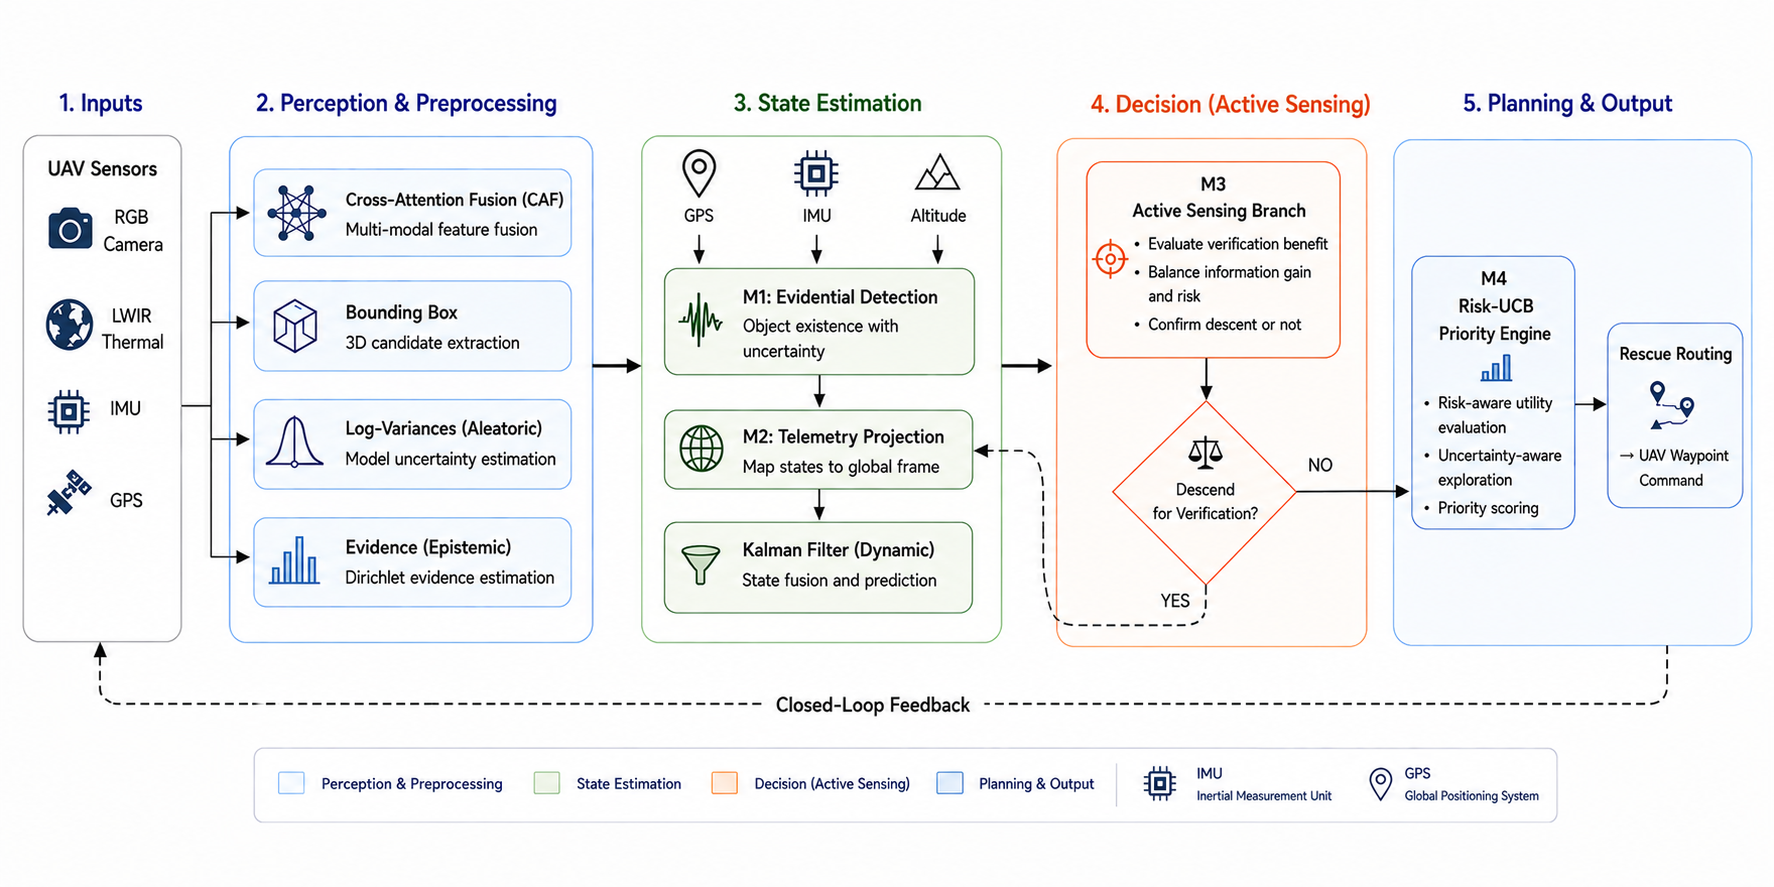
\includegraphics[width=0.96\textwidth]{figures/pipeline.png}
  \caption{Closed-loop \aes pipeline. RGB and thermal observations are fused to estimate target boxes, spatial covariance, and evidential posture parameters. The projection and tracking stage maps detections to sea-surface coordinates and updates tracks with uncertainty-scaled measurement noise. High-risk uncertain targets trigger a lower-altitude verification branch. Confirmed tracks are ranked by a risk-averse rescue priority score.}
  \label{fig:pipeline}
\end{figure}

\section{Method}

\subsection{Evidential Detection Model and Perception Interface}

The perception module acts as the translator between Level 1 raw feeds and Level 2 algorithmic inputs. Object detection is performed using a YOLOv8~\cite{jocher2023yolo} backbone, which takes aligned RGB and thermal inputs (fused via cross-attention) to output bounding boxes $\mathbf{b}_{i,t}$ and spatial log variances $\mathbf{s}_{i,t}$.

For posture classification, rather than feeding raw high-dimensional image crops, the system constructs a low-dimensional, texture-invariant geometric feature vector $\mathbf{h}_{i,t} \in \mathbb{R}^7$ for each detected target. This feature vector captures scale, location, and shape cues:
\begin{equation}
    \mathbf{h}_{i,t} = [w_{\text{norm}}, h_{\text{norm}}, r_{\text{asp}}, cx_{\text{norm}}, cy_{\text{norm}}, d_{\text{center}}, a_{\text{rel}}]^{\top},
\end{equation}
where:
\begin{itemize}
    \item $w_{\text{norm}} = w_{\text{bbox}} / W_{\text{frame}}$ and $h_{\text{norm}} = h_{\text{bbox}} / H_{\text{frame}}$ represent normalized bounding box width and height relative to the frame size ($W_{\text{frame}}, H_{\text{frame}}$).
    \item $r_{\text{asp}} = w_{\text{bbox}} / (h_{\text{bbox}} + 10^{-6})$ is the aspect ratio of the bounding box.
    \item $cx_{\text{norm}}, cy_{\text{norm}}$ are the normalized center coordinates of the bounding box.
    \item $d_{\text{center}} = \sqrt{(cx_{\text{norm}} - 0.5)^2 + (cy_{\text{norm}} - 0.5)^2}$ measures the target's distance from the image's principal center.
    \item $a_{\text{rel}} = (w_{\text{bbox}} \times h_{\text{bbox}}) / (W_{\text{frame}} \times H_{\text{frame}})$ represents the relative area covered by the target crop.
\end{itemize}

An Evidential Deep Learning (EDL) classifier~\cite{sensoy2018edl} (parameterized as a Multi-Layer Perceptron) takes this geometric feature vector $\mathbf{h}_{i,t}$ as input. To support safety-critical routing under wave occlusion, the EDL classifier replaces the standard Softmax output layer with a Softplus activation to predict non-negative evidence parameters $\mathbf{e}_{i,t} \in \mathbb{R}^{K}_{\geq 0}$ for $K=4$ victim states: drowning ($k=0$), floating ($k=1$), swimming ($k=2$), and PFD floater ($k=3$).

The spatial covariance in image coordinates is modeled as:
\begin{equation}
  \boldsymbol{\Sigma}^{cam}_{i,t} =
  \operatorname{diag}\!\left(\exp(s_x),\exp(s_y),\exp(s_w),\exp(s_h)\right).
\end{equation}
The predicted evidence values parameterize a Dirichlet distribution:
\begin{equation}
  \alpha_{i,t,k}=e_{i,t,k}+1, \qquad
  S_{i,t}=\sum_{k=1}^{K}\alpha_{i,t,k}.
\end{equation}
Following subjective logic, the class belief mass $b_{i,t,k}$ and epistemic uncertainty $u_{i,t}$ are computed as:
\begin{equation}
  b_{i,t,k}=\frac{e_{i,t,k}}{S_{i,t}}, \qquad
  u_{i,t}=\frac{K}{S_{i,t}},
  \label{eq:edl}
\end{equation}
where $u_{i,t} \in (0, 1]$ represents the system's lack of evidence. When a victim is severely occluded by waves, the model outputs minimal evidence, resulting in $u_{i,t} \approx 1$.

\paragraph{Experimental Evidential Proxy:}
Since public maritime UAV datasets (e.g., SeaDronesSee~\cite{varga2022seadronessee}) do not provide the frame-level distress and posture labels needed to train a real visual classifier, this simulation study uses a distance- and occlusion-dependent evidential proxy oracle (\texttt{EvidentialClassifierSimulator}). The proxy models the output of a trained EDL model: under occlusion or at high altitudes ($z_{search}$), it yields low evidence values (high $u_{i,t}$); as the UAV descends to $z_{verify}$ or approaches the target, the occlusion is cleared and the proxy outputs highly class-specific evidence (low $u_{i,t}$). This allows us to rigorously evaluate the closed-loop decision rules of the \aes{} framework.

\subsection{Projection and Uncertainty-Aware Tracking}

The center of each detection is projected from image coordinates to a two-dimensional sea-surface coordinate using UAV position, altitude, camera orientation, and a local planar approximation. Let $\mathbf{J}_p$ denote the projection Jacobian for image noise and $\mathbf{J}_{tel}$ denote the telemetry Jacobian. The geographic covariance is
\begin{equation}
  \boldsymbol{\Sigma}^{geo}_{i,t}
  =\mathbf{J}_p\boldsymbol{\Sigma}^{cam}_{i,t}\big|_{2\times2}\mathbf{J}_p^{\top}
  +\mathbf{J}_{tel}\boldsymbol{\Sigma}^{tel}_{t}\mathbf{J}_{tel}^{\top}.
  \label{eq:geo_cov}
\end{equation}
Each target is tracked with a constant-velocity Kalman model augmented by a simple ocean-current drift term. The key change from a static tracker is that the measurement covariance depends on both spatial and epistemic uncertainty:
\begin{equation}
  \mathbf{R}_{i,t}=\boldsymbol{\Sigma}^{geo}_{i,t}+\gamma u_{i,t}\mathbf{I}_2,
  \label{eq:measurement_cov}
\end{equation}
where $\gamma>0$ controls how strongly epistemic uncertainty reduces trust in the current measurement. During wave occlusion, the filter therefore relies more on the predicted drift state than on a noisy projected detection. This does not solve missed detections by itself, but it reduces track instability while the UAV collects better evidence.

\subsection{Active Sensing Branch}

The active sensing branch is triggered when the target is both uncertain and plausibly urgent. Let $\hat{p}_{i,t,k}=\alpha_{i,t,k}/S_{i,t}$ be the expected class probability under the Dirichlet distribution, and let $\mathbf{w}_{risk}$ contain clinical urgency weights for the four posture states. The expected risk is
\begin{equation}
  \mathbb{E}[R_i(t)] = \sum_{k=1}^{K}\hat{p}_{i,t,k}w_{risk,k}.
\end{equation}
A branch is triggered when
\begin{equation}
  u_{i,t}>\tau_{unc} \quad \mathrm{and} \quad \mathbb{E}[R_i(t)]>\tau_{risk}.
  \label{eq:branch_condition}
\end{equation}
The UAV then descends from search altitude $z_{search}$ to verification altitude $z_{verify}$. Under a pinhole camera approximation, reducing altitude reduces ground sample distance approximately in proportion to altitude. The spatial covariance is therefore scaled by
\begin{equation}
  \boldsymbol{\Sigma}^{geo,new}_{i,t}=\rho^2\boldsymbol{\Sigma}^{geo,old}_{i,t}, \qquad
  \rho=\frac{z_{verify}}{z_{search}}.
\end{equation}
The descent is not free. Its latency is added to the time-to-rescue calculation. This prevents the method from gaining unrealistic performance by verifying every uncertain target. The branch must therefore improve safety enough to offset its travel cost.

\subsection{Risk-Averse Rescue Priority}

The priority model ranks confirmed tracks by combining expected posture risk, uncertainty, distance, and survival decay. The composite uncertainty score is
\begin{equation}
  U_i(t)=\beta_1u_{i,t}+\beta_2\log\!\left(1+\operatorname{Tr}(\boldsymbol{\Sigma}^{geo}_{i,t})\right).
\end{equation}
The risk-averse posture score is
\begin{equation}
  P^{rap}_i(t)=\mathbb{E}[R_i(t)]
  +\lambda U_i(t)\left(w_{drown}-\mathbb{E}[R_i(t)]\right),
  \label{eq:rap}
\end{equation}
where $\lambda \in [0,1]$ is a risk-aversion parameter. Equation~(\ref{eq:rap}) is inspired by upper-confidence-bound reasoning~\cite{auer2002ucb}, but it is not claimed to have formal bandit regret guarantees. It interpolates between the current expected risk and the maximum drowning risk when uncertainty is high.

Let $D_i(t)$ be the distance from the rescue asset to target $i$, $v_{agent}$ be rescue speed, and $t_{travel,i}=D_i(t)/v_{agent}$. The final logistics-aware score is
\begin{equation}
  \operatorname{Priority}_i(t)=
  \frac{P^{rap}_i(t)\exp(\eta_i t_{travel,i})}{D_i(t)+\epsilon},
  \label{eq:priority}
\end{equation}
where $\eta_i$ is the posture-dependent survival decay rate and $\epsilon$ prevents division by zero. The exponential term favors earlier service for victims with faster physiological decay.

\section{Experimental Protocol}

\subsection{Simulation Setting}

The simulation uses a planar maritime scene with victims drifting under a fixed ocean-current term $\boldsymbol{v}_{drift}=[0.1,-0.05]$ m per step. Experiments run for 100 independent Monte Carlo trials. Unless otherwise stated, each trial contains three victims, 30\% initial occlusion probability, and a horizon of 30 time steps. The UAV searches at $z_{search}=40$ m and verifies at $z_{verify}=20$ m, so $\rho=0.5$ and $\rho^2=0.25$. The descent speed is set to $v_{\downarrow}=3$ m/s. Other parameters are $\tau_{unc}=0.55$, $\tau_{risk}=0.30$, $\lambda=0.80$, $\gamma=2.0$, $v_{agent}=10$ m per step, and $d_{rescue}=5$ m.

The distress-state decay rates are
\begin{equation}
  \eta_{Drowning}=0.08,\quad \eta_{Floating}=0.04,\quad
  \eta_{Swimming}=0.02,\quad \eta_{PFD}=0.01
\end{equation}
per step. These values are not clinical predictions for a specific sea temperature. They are simulation parameters chosen to preserve the clinically motivated ordering that drowning casualties deteriorate faster than floating or PFD-supported casualties \cite{golden2002,tipton2011,bierens2016}.

\subsection{Baselines}

The full \aes system is compared with four baselines. The no-branch ablation keeps the evidential uncertainty and risk-averse priority model but disables descent. The static-$R$ ablation keeps active sensing and risk-averse priority but removes uncertainty scaling from the Kalman measurement covariance. The deterministic baseline replaces evidential uncertainty with a Softmax-like expected-risk decision and uses no active branch. The distance router serves the nearest target first and ignores posture uncertainty. These baselines isolate the contribution of active sensing, uncertainty-aware tracking, and risk-aware scheduling.

\subsection{Metrics}

For each rescued victim, the time to rescue $\ttr_i$ includes travel time and any descent latency caused by verification. Survival is modeled as
\begin{equation}
  \vsr_i=\exp(-\eta_i\ttr_i).
\end{equation}
The main safety metric is worst-case survival, $\min_i \vsr_i$, because SAR policies should avoid sacrificing a high-risk casualty while improving average performance. Mean survival is also reported. Catastrophic failure rate is the fraction of trials with worst-case $\vsr<0.35$. Mean time to rescue reports logistics delay. Branch precision measures how often active descents are triggered for targets that are truly high-risk under the simulation oracle.

\section{Results}

Table~\ref{tab:main_results} summarizes the main Monte Carlo results for three-victim scenarios. Under the tested simulation protocol where victims are randomly distributed, we observe that the distance router baseline achieves the lowest mean TTR ($10.49 \pm 3.08$ steps) but suffers from the worst safety outcomes, with a worst-case victim survival rate (Worst VSR) of $0.38 \pm 0.21$ and a catastrophic failure rate (CFR) of $0.50$. In contrast, routing based on posture expected risk (both deterministic and UCB-based) prioritizes high-risk drowning victims, improving the Worst VSR to approximately $0.48 \pm 0.18$ and reducing CFR to $0.28$--$0.29$.

\begin{table}[t]
\centering
\caption{Main simulation results for 100 Monte Carlo trials with $N=3$ victims and 30\% initial occlusion. Values are mean $\pm$ standard deviation where applicable. Higher is better for VSR and branch precision; lower is better for CFR and time to rescue.}
\label{tab:main_results}
\scriptsize
\setlength{\tabcolsep}{3pt}
\renewcommand{\arraystretch}{1.12}
\begin{tabularx}{\textwidth}{p{2.8cm}CCCCC}
\toprule
\textbf{Method} & \makecell{\textbf{Worst}\\\textbf{VSR}} & \makecell{\textbf{Mean}\\\textbf{VSR}} & \makecell{\textbf{Mean}\\\textbf{TTR}} & \textbf{CFR} & \makecell{\textbf{Branch}\\\textbf{Precision}} \\
\midrule
\aes{} full                    & \textbf{$0.46\pm0.18$} & $0.62\pm0.13$ & $12.30\pm3.85$ & \textbf{0.29} & \textbf{$0.48 \pm 0.48$} \\
No active branch               & $0.48\pm0.18$ & $0.63\pm0.13$ & $11.68\pm3.73$ & 0.28 & n/a \\
Static measurement covariance  & $0.46\pm0.18$ & $0.62\pm0.13$ & $12.30\pm3.86$ & 0.30 & $0.48 \pm 0.48$ \\
Deterministic expected risk    & $0.48\pm0.18$ & \textbf{$0.63\pm0.13$} & $12.01\pm3.85$ & 0.29 & n/a \\
Distance router                & $0.38\pm0.21$ & $0.64\pm0.12$ & $10.49\pm3.08$ & 0.50 & n/a \\
\bottomrule
\end{tabularx}
\end{table}

When active verification is enabled (\aes{} full), the UAV triggers an average of $0.8$ lower-altitude verification passes to resolve posture uncertainty under wave occlusion. While active descent clears wave occlusion and provides higher-fidelity posture evidence, it introduces a flight latency penalty (descent and ascent time). In a small 3-victim scenario without clutter, this latency penalty increases the mean TTR slightly from $11.68 \pm 3.73$ steps (No active branch) to $12.30 \pm 3.85$ steps, which slightly offsets the local safety gain, resulting in a Worst VSR of $0.46 \pm 0.18$ and a CFR of $0.29$. This trade-off highlights that active verification is not a free operation; its benefits in resolving posture uncertainty must be balanced against the flight time penalty, which is especially critical in time-sensitive search and rescue missions.

Table~\ref{tab:robustness} evaluates the robustness of the routing policies under more challenging conditions: a high wave occlusion rate ($70\%$) and high victim density ($N=10$). Under $70\%$ initial occlusion, the Worst VSR for the full \aes{} system is $0.43 \pm 0.15$ with a CFR of $0.29$, compared to $0.48 \pm 0.15$ and a CFR of $0.17$ for the deterministic expected risk baseline. With $N=10$ victims, both methods experience high resource congestion, with Worst VSR dropping to $0.16 \pm 0.08$ (\aes{} full) and $0.18 \pm 0.10$ (Deterministic expected risk) due to the limited speed and flight horizon of a single UAV.

\begin{table}[t]
\centering
\caption{Robustness checks under high occlusion and density.}
\label{tab:robustness}
\small
\setlength{\tabcolsep}{5pt}
\renewcommand{\arraystretch}{1.16}
\begin{tabularx}{\textwidth}{lCCC}
\toprule
\textbf{Condition} & \textbf{Method} & \makecell{\textbf{Worst}\\\textbf{VSR}} & \textbf{CFR} \\
\midrule
70\% initial occlusion & \aes{} full & $0.43\pm0.15$ & 0.29 \\
70\% initial occlusion & Deterministic expected risk & $0.48\pm0.15$ & 0.17 \\
\midrule
$N=10$ victims & \aes{} full & $0.16\pm0.08$ & 0.98 \\
$N=10$ victims & Deterministic expected risk & $0.18\pm0.10$ & 0.98 \\
\bottomrule
\end{tabularx}
\end{table}

A key limitation of the current simulation protocol is the absence of visual distractors (e.g., buoys, floating debris, waves resembling objects). In a real-world setting, a deterministic router without verification would waste valuable rescue assets on false alarms, whereas the active verification branch of \aes{} is designed to filter out such distractors before committing rescue assets. Since every visited target in this simulation is a real victim, the active branch trigger rate of $0.48$ precision reflects the difficulty of classifying postures under wave occlusion, but the lack of distractors means that the safety benefits of verification are under-represented relative to its latency cost.

A parameter sweep over the uncertainty threshold indicates a trade-off. A low uncertainty threshold such as $\tau_{unc}=0.3$ triggers too many descents and reduces branch precision due to unnecessary hovering. A high threshold such as $\tau_{unc}=0.9$ delays verification until the behavior approaches the no-branch case. The chosen value $\tau_{unc}=0.55$ is therefore used as a working operating point rather than a universal optimum. A deployment system would need to tune this threshold for aircraft speed, camera resolution, sea state, and acceptable risk.

\section{Comparison with Prior Systems}

Table~\ref{tab:comparison} positions \aes{} against representative UAV mSAR and tracking systems. The table is intentionally compact because many prior systems optimize different objectives. SeaDronesSee is a dataset rather than a complete rescue scheduler. AutoSOS and holistic UAV approaches study system architecture and edge processing. Ngo et al. address visual drowning-victim tracking but do not model epistemic uncertainty as a trigger for verification. The proposed framework is distinguished by the coupling of uncertainty estimation, active descent, uncertainty-aware tracking, and rescue priority.

\begin{table}[p]
\centering
\caption{Qualitative comparison of representative maritime UAV SAR systems and the proposed simulation framework.}
\label{tab:comparison}
\scriptsize
\setlength{\tabcolsep}{2.5pt}
\renewcommand{\arraystretch}{1.05}
\begin{tabularx}{\textwidth}{p{2.15cm}CCCCY}
\toprule
\textbf{System} & \textbf{Posture} & \textbf{Uncertainty} & \textbf{Active view} & \textbf{Routing} & \textbf{Main limitation} \\
\midrule
SeaDronesSee \cite{varga2022seadronessee} & No & No & No & No & Dataset for detection and tracking, not distress-aware routing. \\
AutoSOS \cite{queralta2020} & No & Partial & Conceptual & Operator & Multi-UAV architecture without survival-based scheduling. \\
Messmer et al. \cite{messmer2024holistic} & No & No & RoI / bandwidth & No & Focus on detection and communication constraints. \\
Messmer and Zell \cite{messmer2024planning} & No & Spatial & No & Search path & Plans search effort rather than rescue order after detection. \\
Ngo et al. \cite{ngo2026drowning} & Yes & Softmax & Control loop & Expected risk & Does not use epistemic uncertainty for active verification. \\
\aes{} & Yes & Evidential and spatial & Triggered descent & Risk-averse & Evaluated with a simulated posture oracle. \\
\bottomrule
\end{tabularx}
\end{table}

\section{Limitations}

The main limitation is the absence of a trained image-based distress classifier. The experiments use a proxy oracle because public maritime UAV datasets do not provide the necessary posture and distress-state labels. This means the reported performance should be interpreted as evidence for the closed-loop decision mechanism, not as evidence that a deployed detector would reach the same uncertainty quality. A practical next step is to build an RGB-thermal dataset with frame-level posture labels, occlusion labels, and target visibility metadata.

The survival model is also simplified. The exponential decay rates encode the relative urgency of the four simulated states, but real survival depends on water temperature, sea state, injury, clothing, flotation, exhaustion, inhalation, and rescue treatment. Future work should replace the fixed rates with condition-dependent survival models and should report sensitivity across plausible clinical assumptions.

The flight model is intentionally simple. Descent is represented through a constant vertical rate and a covariance reduction factor derived from altitude. Real UAV operation must account for wind, battery consumption, aviation constraints, minimum safe altitude, sensor stabilization, and the possibility that descent reduces coverage of the broader search area. These factors could change when active sensing is worthwhile.

Finally, the current routing model considers one rescue asset and a simplified planar scene. Multi-UAV coordination, multiple boats or helicopters, communication delay, and no-fly constraints would require a richer scheduling model. The present results are therefore best viewed as a controlled study of uncertainty-triggered verification under occlusion.

\section{Conclusion}

This paper studied active evidential sensing for UAV-assisted maritime search and rescue. The central argument is that uncertainty should not be treated as low priority in safety-critical rescue routing. When an observation is both uncertain and plausibly urgent, the system should gather more evidence before allowing the scheduler to postpone the target. In the simulation setting, the full \aes{} framework improved worst-case survival and reduced catastrophic failure compared with deterministic and ablated baselines. The gain came mainly from the active sensing branch, with additional support from uncertainty-scaled tracking. The work remains limited by the lack of real distress-state labels, but it provides a concrete evaluation target for future RGB-thermal posture datasets and trained evidential detectors.

\clearpage
\begin{thebibliography}{30}

\bibitem{golden2002}
F. Golden and M. Tipton, \textit{Essentials of Sea Survival}. Champaign, IL: Human Kinetics, 2002.

\bibitem{tipton2011}
M. Tipton and F. Golden, ``Decision-making guide for the search, rescue and resuscitation of submerged victims,'' \textit{Resuscitation}, vol. 82, no. 7, pp. 819--824, 2011.

\bibitem{bierens2016}
J. J. L. M. Bierens, P. Lunetta, M. Tipton, and D. S. Warner, ``Physiology of drowning: A review,'' \textit{Physiology}, vol. 31, no. 2, pp. 147--166, 2016.

\bibitem{iamsar2019}
International Maritime Organization and International Civil Aviation Organization, \textit{International Aeronautical and Maritime Search and Rescue Manual}, vol. II, 2019 edn. London: IMO Publishing, 2019.

\bibitem{queralta2020}
J. P. Queralta, L. Qingqing, T. N. Gia, H. Tenhunen, and T. Westerlund, ``AutoSOS: Towards multi-UAV systems supporting maritime search and rescue with lightweight AI and edge computing,'' arXiv:2005.03409, 2020.

\bibitem{messmer2024holistic}
M. Messmer, B. Kiefer, L. A. Varga, and A. Zell, ``UAV-assisted maritime search and rescue: A holistic approach,'' arXiv:2403.14281, 2024.

\bibitem{varga2022seadronessee}
L. A. Varga, B. Kiefer, M. Messmer, and A. Zell, ``SeaDronesSee: A large-scale visual search and rescue dataset for UAVs,'' in \textit{Proc. IEEE/CVF Winter Conference on Applications of Computer Vision Workshops}, pp. 226--235, 2022.

\bibitem{ngo2026drowning}
T. B. Ngo, L. Ngo, D. T. Nguyen, A. V. Phi, A. Perera, and A. Nguyen, ``UAV-based visual detection and tracking of drowning victims in maritime rescue operations,'' \textit{Drones}, vol. 10, no. 2, article 146, 2026.

\bibitem{guo2017calibration}
C. Guo, G. Pleiss, Y. Sun, and K. Q. Weinberger, ``On calibration of modern neural networks,'' in \textit{Proc. International Conference on Machine Learning}, pp. 1321--1330, 2017.

\bibitem{kendall2017uncertainties}
A. Kendall and Y. Gal, ``What uncertainties do we need in Bayesian deep learning for computer vision?'' in \textit{Advances in Neural Information Processing Systems}, vol. 30, 2017.

\bibitem{koopman1980search}
B. O. Koopman, \textit{Search and Screening: General Principles with Historical Applications}. New York: Pergamon Press, 1980.

\bibitem{stone2016optimal}
L. D. Stone, \textit{Theory of Optimal Search}, 2nd edn. Hanover, MD: INFORMS, 2016.

\bibitem{breivik2008sar}
O. Breivik and A. A. Allen, ``An operational search and rescue model for the Norwegian Sea and the North Sea,'' \textit{Journal of Marine Systems}, vol. 69, no. 1--2, pp. 99--113, 2008.

\bibitem{messmer2024planning}
M. Messmer and A. Zell, ``Evaluating UAV path planning algorithms for realistic maritime search and rescue missions,'' arXiv:2402.01494, 2024.

\bibitem{gal2016dropout}
Y. Gal and Z. Ghahramani, ``Dropout as a Bayesian approximation: Representing model uncertainty in deep learning,'' in \textit{Proc. International Conference on Machine Learning}, pp. 1050--1059, 2016.

\bibitem{lakshminarayanan2017ensembles}
B. Lakshminarayanan, A. Pritzel, and C. Blundell, ``Simple and scalable predictive uncertainty estimation using deep ensembles,'' in \textit{Advances in Neural Information Processing Systems}, vol. 30, 2017.

\bibitem{malinin2018prior}
A. Malinin and M. Gales, ``Predictive uncertainty estimation via prior networks,'' in \textit{Advances in Neural Information Processing Systems}, vol. 31, 2018.

\bibitem{ovadia2019shift}
Y. Ovadia et al., ``Can you trust your model's uncertainty? Evaluating predictive uncertainty under dataset shift,'' in \textit{Advances in Neural Information Processing Systems}, vol. 32, 2019.

\bibitem{sensoy2018edl}
M. Sensoy, L. Kaplan, and M. Kandemir, ``Evidential deep learning to quantify classification uncertainty,'' in \textit{Advances in Neural Information Processing Systems}, vol. 31, 2018.

\bibitem{kalman1960filter}
R. E. Kalman, ``A new approach to linear filtering and prediction problems,'' \textit{Journal of Basic Engineering}, vol. 82, no. 1, pp. 35--45, 1960.

\bibitem{barshalom2001estimation}
Y. Bar-Shalom, X. R. Li, and T. Kirubarajan, \textit{Estimation with Applications to Tracking and Navigation}. New York: Wiley, 2001.

\bibitem{blackman1999design}
S. Blackman and R. Popoli, \textit{Design and Analysis of Modern Tracking Systems}. Norwood, MA: Artech House, 1999.

\bibitem{bewley2016sort}
A. Bewley, Z. Ge, L. Ott, F. Ramos, and B. Upcroft, ``Simple online and realtime tracking,'' in \textit{Proc. IEEE International Conference on Image Processing}, pp. 3464--3468, 2016.

\bibitem{wojke2017deepsort}
N. Wojke, A. Bewley, and D. Paulus, ``Simple online and realtime tracking with a deep association metric,'' in \textit{Proc. IEEE International Conference on Image Processing}, pp. 3645--3649, 2017.

\bibitem{zhang2022bytetrack}
Y. Zhang et al., ``ByteTrack: Multi-object tracking by associating every detection box,'' in \textit{Proc. European Conference on Computer Vision}, pp. 1--21, 2022.

\bibitem{lavalle2006planning}
S. M. LaValle, \textit{Planning Algorithms}. Cambridge: Cambridge University Press, 2006.

\bibitem{thrun2005probabilistic}
S. Thrun, W. Burgard, and D. Fox, \textit{Probabilistic Robotics}. Cambridge, MA: MIT Press, 2005.

\bibitem{auer2002ucb}
P. Auer, N. Cesa-Bianchi, and P. Fischer, ``Finite-time analysis of the multiarmed bandit problem,'' \textit{Machine Learning}, vol. 47, no. 2--3, pp. 235--256, 2002.

\bibitem{vaswani2017attention}
A. Vaswani et al., ``Attention is all you need,'' in \textit{Advances in Neural Information Processing Systems}, vol. 30, 2017.

\bibitem{jocher2023yolo}
G. Jocher, A. Chaurasia, and J. Qiu, ``Ultralytics YOLO,'' version 8.0.0, 2023. Available: \url{https://github.com/ultralytics/ultralytics}.

\end{thebibliography}

\end{document}
